\section{Problem formulation}
\label{sec:formulation}
In this section we derive fast, almost exact projector for 3D cone beam geometry. We use linear Lambert-Beer law to compute pixel signal based on the known function $\mu : \mathbb{R}^3 \to \mathbb{R}^+_0 $ that represents the attenuation. We emphasize that instead of direct integration of the attenuation over the rays to the detector we find a mathematical transformation to integrate attenuation over the subvolumes of voxels projected to given pixel.

\subsection{Geometry discretization}
Throughout the paper, we will use the following standard assumptions about the discretized problem. Let's the X-ray source, object to be scanned and the detector be located in the Euclidean space $\mathbb{R}^3$. The X-ray source at given time $t$ has coordinates  $\vec{s} = (s_1, s_2, s_3)$. The object to be scanned lies inside a rectangular box $V$ centered at $(0,0,0)$ with the edge lengths $(l_1, l_2, l_3) \in \mathbb{R}_{+}^3$. Box $V$ represents the volume to be projected
\begin{equation}
    V = \{ \vec{x} \in \mathbb{R}^3 : |x_1| < \frac{l_1}{2},|x_2| < \frac{l_2}{2}, |x_3| < \frac{l_3}{2} \}.
    \nonumber
\end{equation}
The discretization is given by the voxel sizes $(a_1,a_2,a_3) \in \mathbb{R}_{+}^3$ and number of the voxels per edge $(N_1, N_2, N_3) \in \mathbb{N}^3$. For the dimension compatibility it is required that $a_\alpha N_\alpha = l_\alpha$ for $\alpha \in \{1,2,3\}$. Let's denote the center of the voxel $(0,0,0)$ by 
\begin{equation}
    \vec{x}^{(0,0,0)} =  (\frac{-l_1 + a_1}{2}, \frac{-l_2 + a_2}{2}, \frac{-l_3+a_3}{2}).
    \nonumber
\end{equation}
The center of the general voxel $(i,j,k)$,  $i\in \{0...N_1-1\}$, $j\in \{0...N_2-1\}$ and $k\in \{0...N_3-1\}$ is then
\begin{equation}
    \vec{x}^{(i,j,k)} = \vec{x}^{(0,0,0)} +  (i a_1, j a_2, k a_3),
    \nonumber
\end{equation}
and the volume of the voxel is given by
\begin{equation}
V^{(i,j,k)} = \{ \vec{x} \in \mathbb{R}^3 : |x_\alpha-x^{(i,j,k)}_\alpha| < \frac{a_\alpha}{2}, \alpha \in \{1,2,3\} \}.
\nonumber
\end{equation}
The attenuation $\mu : \mathbb{R}^3 \to \mathbb{R}^+_0 $  has a support on $V$ and is constant on each voxel so that
\begin{equation}
\forall \vec{x} \in V^{(i,j,k)} \quad \mu(\vec{x}) = \mu^{i,j,k}.
\nonumber
\end{equation}

\subsection{Detector discretization}
In what follows, we consider flat panel detector with the rectangle shaped pixels without gaps. Detector surface is parametrized by means of two Euclidean coordinates $\chi = (\chi_1, \chi_2) \in \mathbb{R}^2$. These assumptions allow us to clearly explain main concepts, yet it is straightforward to relax them and consider curved detectors, differently shaped pixels and gaps between pixels. In the current implementation, to compute the cuts, we additionally assume that the $x_3$ axis of the global geometry is parallel to the $\chi_2$ axis of the detector, see Figure \ref{fig:carmconventionalsetup}. However, this assumption is not essential to derive the main formula for the cutting voxel projector in this chapter.

Let's assume that $(M, N) \in \mathbb{N}^2$ are the counts of the pixels per edge and the spacing of pixels is given by $(b_1,b_2) \in \mathbb{R}_{+}^2$. The center of the pixel $(0,0)$ is $\vec{\chi}^{(0,0)} =  (0, 0)$. The center of the general pixel $(m,n)$,  $m\in \{0...M-1\}$ and $n\in \{0...N-1\}$ is at
\begin{equation}
    \vec{\chi}^{(m,n)} = \vec{\chi}^{(0,0)} +  (m b_1, n b_2)
\end{equation}
and the surface of the pixel is parametrized as
\begin{equation}
A^{(m,n)} = \{ \vec{\chi} : |\chi_\alpha-\chi^{(m,n)}_\alpha| < \frac{b_\alpha}{2}, \alpha \in \{1,2\} \}.
\end{equation}

\subsection{Parametrization of the rays and attenuation model}

To define the geometry of the system, we begin by fixing the positions of the source and detector. Using these fixed points, we introduce a spherical coordinate system denoted by $(r, \theta, \varphi) \in [0,\infty] \times [0,\pi/2] \times [0,2\pi)$, which which originates at the source position and provides a natural way to describe the rays from the source to the particular detector position. The zenith denotes the direction with zero inclination $\theta = 0$, which corresponds to the principal ray that is the ray orthogonal to the flat panel detector. The intersection of the detector with the principal ray is called the principal point $\vec{\chi}^{P} =  (\chi_1^P, \chi_2^P)$. Rays with azimuth $\varphi = 0$ are projected onto a semi-line on the detector starting at a principal point parallel to the $\chi_1$ axis.

For a given view, there is an exact correspondence between this local spherical coordinate system and the global coordinate system. We can introduce an auxiliary Euclidean system $(\tilde{x}_1, \tilde{x}_2, \tilde{x}_3)$ centered at $\vec{s}$ and the transformation given by orthogonal $3 \times 3$ matrix $Q$ such that 
\begin{equation}
    \tilde{\vec{x}} = Q (\vec{x} - \vec{s}).
\end{equation}
The rotation $Q$ transforms the axes so that $x_1$ is parallel to the detector coordinate $\chi_1$, $x_2$ is parallel to $\chi_2$ and $x_3$ is in the direction of the normal from the source to the detector, see Figure \ref{fig:flat_panel}.
The system $(\tilde{x}_1, \tilde{x}_2, \tilde{x}_3)$ then in turn induces local spherical coordinate system in a way that
\begin{align}
    r &= \sqrt{\tilde{x}_1^2 + \tilde{x}_2^2 + \tilde{x}_3^2},\\
    \theta &= \arccos \frac{\tilde{x}_3}{\sqrt{\tilde{x}_1^2 + \tilde{x}_2^2 + \tilde{x}_3^2}},\\
    \varphi &= \atantwo (\tilde{x}_2, \tilde{x}_1).
\end{align}

\begin{figure}
    \centering
    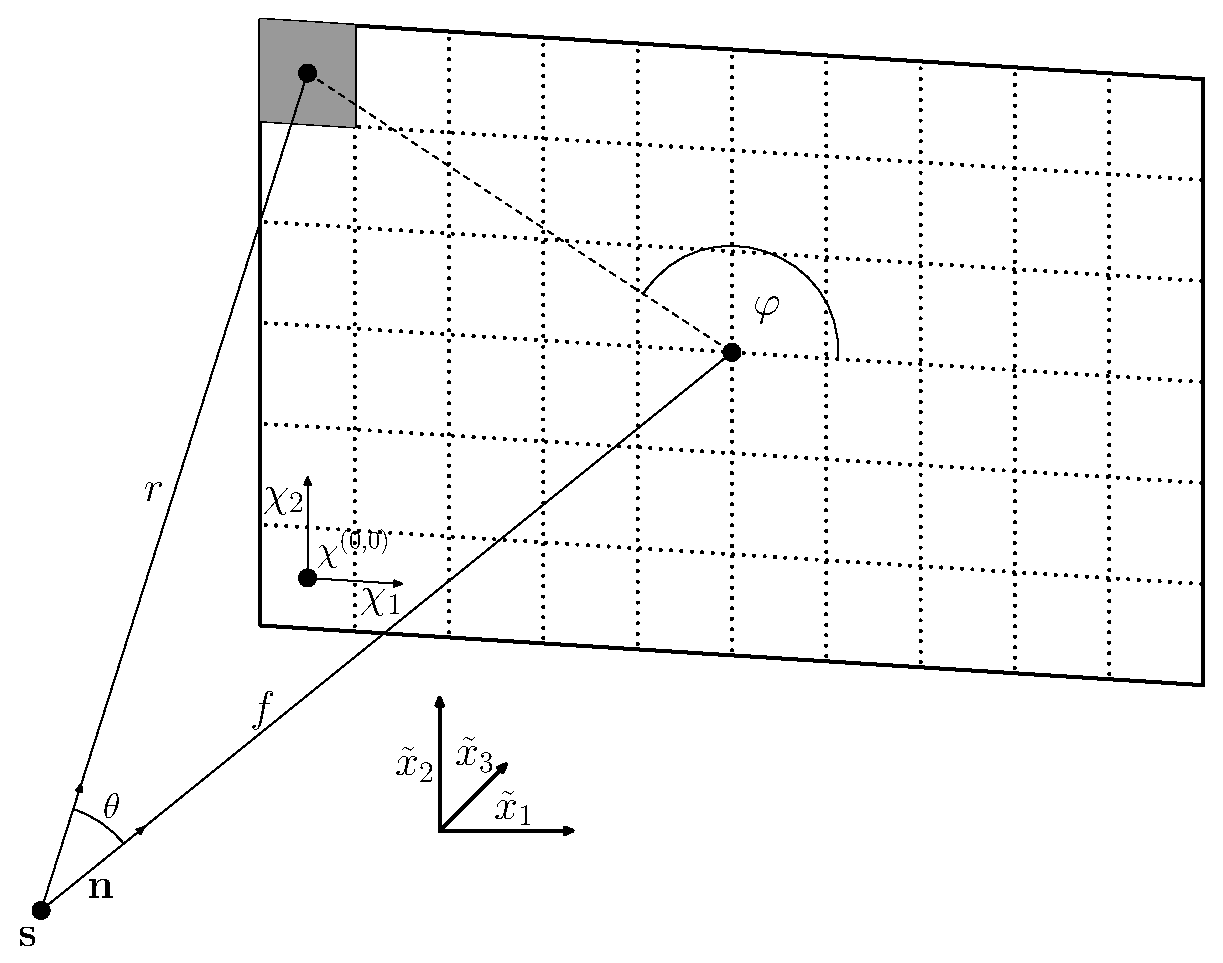
\includegraphics[width=0.45\textwidth]{auxiliaryLocalCoordinatesV05.eps}
    \caption{Auxiliary local Euclidean coordinates for a given view that induce a local spherical coordinate system. Coordinate $\theta$ is the cone angle.}
    \label{fig:flat_panel}
\end{figure}

The model given by Lambert-Beer law and the cone beam geometry maps the lines in $\mathbb{R}^3$ starting at the source position $\vec{s}$ to the integrals over the attenuation $\mu$ along these lines. The lines can be parametrized by polar and azimuthal angles in spherical coordinate system $[\theta, \varphi] \in [-\pi/2,\pi/2] \times [0,2\pi)$. Let's $\vec{L}[\theta, \varphi]: \mathbb{R} \to \mathbb{R}^3$ define a isometric parametrization $\vec{L}[\theta, \varphi](q), q \in [0, \infty)$ of the ray  in the direction $[\theta, \varphi]$ such that $\vec{L}[\theta, \varphi](0) = \vec{s}$. 

We identify the coordinates $\chi = (\chi_1, \chi_2) \in \mathbb{R}^2$ with the parameters $\theta,\varphi$, which define the line line through the source $L[\theta,\varphi](.)$ that hits the detector at $(\chi_1, \chi_2)$. 
We consider $[\theta,\varphi]$ or $[\chi_1, \chi_2]$ just two different parametrizations of the  set of all lines passing through the $\vec{s}$. In the projective geometry such set is called projective plane or projective space of dimension two, see \cite{Prasolov2001}.

Consider the ray in the direction $[\theta, \varphi]$. According to Lambert-Beer law the X-ray intensity after passing the scanned object measured on the detector is
\begin{equation}
    I(\theta, \varphi) = I_0(\theta, \varphi) \exp{\left(-\INTEGRAL{_0^\infty}{\mu(\vec{L}[\theta, \varphi]( q))}{q}\right)}, \label{eq:lambertbeer}
\end{equation}
where $I_0(\theta, \varphi)$ is the blank scan intensity that would be measured at the same detector position without scanned object. The quantity
\begin{equation}
    E(\theta, \varphi) \stackrel{1}{=} \ln(I_0(\theta, \varphi)) - \ln(I(\theta, \varphi)) \stackrel{2}{=} \INTEGRAL{_0^\infty}{ \mu(\vec{L}(\theta, \varphi, q))}{q}
    \label{eq1:extinciton}
\end{equation}
is in what follows called \textbf{extinction}. It is not common terminology and sometimes it is refereed just as negative logarithm of transmission or line integral of attenuation. When referring to the discretized tomographic problem \eqref{eq:fundament}, we call discretized extinction often right hand side, projection vector or vector $\vec{b}$.

\subsection{Per pixel extinction}
\label{sec:perpixel}
When scanning the volume $V$, the CT scanner measures the intensities $I^{(m,n)}$ for each view and each pixel on the detector and and then calculates the extinction values $E^{(m,n)}$ based on the known per pixel intensities $I_0^{(m,n)}$ and the first relation in \eqref{eq1:extinciton}. The values of $E^{(m,n)}$ represent the input vector $\vec{b}$ of the reconstruction problem \eqref{eq:fundament}. In order to obtain specific values within the matrix $\mathbf{A}$, the so-called geometric factors, we need to determine the specific form of the second equation in \eqref{eq1:extinciton} for the discretized extinction $E^{(m,n)}$.

A first order approximation of the relationship between voxel and pixel values is to cast rays towards the pixels and construct the CT operator as follows
\begin{equation}
    E^{(m,n)} = \sum_{i,j,k} \mu^{i,j,k} |V^{(i,j,k)} \cap \vec{L}(\chi^{(m,n)}, .))|,
    \label{eq1:discreteextinction}
\end{equation}
where $|V^{(i,j,k)} \cap \vec{L}(\chi^{(m,n)}, .))|$ is the length of the path of given ray through the given voxel. For computing these intersections, we utilize Siddon algorithm, see \cite{Siddon1985}. The problem with this approach is that the extinction value $E^{(m,n)}$ depends on the exact location on the pixel surface where the beam is cast. The solution is, for example, to create a grid of $K \times K$ equally spaced points on the pixel surface and average all extinction values in \eqref{eq1:discreteextinction} with respect to the rays thrown towards the grid points. We will henceforth refer to the algorithm obtained in this way as \texttt{SiddonK}, i.e., for example, \texttt{Siddon8} casts 64 rays towards each pixel.

To robustly estimate the extinction over pixels, we use the following formula using the integral over the pixel area, which can also be obtained as a limit process derived from the sum over grid points in the \texttt{SiddonK} algorithm if we send $K$ to infinity.
\begin{equation}
    E^{(m,n)} = \frac{e^{(m,n)}}{a^{(m,n)}},\label{eq1:integ}
\end{equation}
where
\begin{equation}
    e^{(m,n)} = \int_{\chi \in A^{(m,n)}} \sum_{i,j,k} \mu^{i,j,k} \mathcal{D}(\chi, i, j, k)  \,dS(\chi), \label{eq1:voxat}
\end{equation}
is the total extinction over the area of the pixel,
\begin{equation}
\mathcal{D}(\chi, i, j, k)  = |V^{(i,j,k)} \cap \vec{L}(\chi, .))|
\end{equation}
is the length of the path of the ray parametrized by $\chi$ through voxel $(i,j,k)$ and
\begin{equation}
    a^{(m,n)} = \int_{\chi \in A^{(m,n)}} 1  \,dS(\chi).
    \label{eq:area}
\end{equation}
The integrals \eqref{eq1:voxat} and \eqref{eq:area} are over the parameterization $\,dS(\chi)$ of the infinitesimal detector surface at point $\chi$ in world coordinates, so that $a^{(m,n)}$ is the area of a given pixel.

Alternatively, we can transform the problem to the unit ball. As we noted $(\theta, \varphi)$ can be also understood as a discretization of unit ball centered at the source position $\vec{s}$. Therefore for given pixel we can integrate \eqref{eq1:extinciton} along $(\theta, \varphi)$ that maps to a given pixel and divide by the surface of the unit ball that maps to that pixel. We have the formula
\begin{equation}
    \bar{E}^{(m,n)} = \frac{\bar{e}^{(m,n)}}{\bar{a}^{(m,n)}},\label{eq1:integub}
\end{equation}
where
\begin{equation}
    \bar{e}^{(m,n)} = \int\limits_{(\theta, \varphi) \in A^{(m,n)}}  \sum_{i,j,k} \mu^{i,j,k} \mathcal{D}(\theta, \varphi, i, j, k) \sin\theta \mathrm{d}\theta \mathrm{d}\varphi \label{eq1:voxatub}
\end{equation}
is the total extinction over the area of the unit ball segment
\begin{equation}
    \bar{a}^{(m,n)} = \int\limits_{(\theta, \varphi) \in A^{(m,n)}}  \sin\theta d\,\theta d\,\varphi.\label{eq1:voxsurfub}
\end{equation}
Here we utilize formula for the unit ball surface element being $dS = \sin\theta d\,\theta d\,\varphi$. 


\subsection{Cutting voxel projector}

To derive new strategy to compute \eqref{eq1:integ} or \eqref{eq1:integub}, we transform integrals over the area of detector cells in \eqref{eq1:voxat} and \eqref{eq1:voxatub} into the integrals over the volume of the voxels of the type
\begin{equation}
    \int_V \mu(\vec{x})\,dx. \label{eqx:volint}
\end{equation}
Using this approach, instead of averaging the ray path length over a voxel, we can then calculate the voxel volume projected onto a given pixel and derive the extinction increment from this value. We start by rewriting the integral \eqref{eq1:voxat} into the form
\begin{equation}
    e^{(m,n)} = \sum_{i,j,k} \mu^{i,j,k} e_{i,j,k}^{(m,n)},
\end{equation}
where
\begin{equation}
     e_{i,j,k}^{(m,n)} = \int_{\chi \in A^{(m,n)}}  |V^{(i,j,k)} \cap \vec{L}(\chi, .)| \,dS(\chi).\label{eq1:svi}
\end{equation}
Let's define an indicator function that tests if the line at the point given by the local spherical coordinates introduced in Figure \ref{fig:flat_panel}, intersects the voxel
\begin{equation}
\vec{I}^{i,j,k}(r, \theta, \varphi) = 
\begin{cases} 1 \quad \mbox{if } \vec{L}(\theta, \varphi, r) \in V^{(i,j,k)} \\
0 \quad \mbox{elsewhere.} \end{cases}
\label{eq:indicator}
\end{equation}
Applying \eqref{eq:indicator}, we rewrite the length of the voxel ray intersection in \eqref{eq1:svi} as
\begin{equation}
    |V^{(i,j,k)} \cap \vec{L}(\chi, .)| = \int_0^\infty \vec{I}^{i,j,k}(r, \theta(\chi), \varphi(\chi)) d\,r.
    \label{eq:rayintegral}
\end{equation}
The surface element in spherical coordinates is $\mathrm{d}\tilde{S}(\chi) = R^2 \sin{\theta} \,\mathrm{d}\theta \,\mathrm{d}\varphi$, where $R$ is the distance of a given pixel on the detector from the source. We assume that the pixel is small enough so that $R$ over its  area can be approximated by a constant value, and also that the curvature of the spherical coordinates on its surface can be ignored so that the angle between the pixel and the element $\mathrm{d}\tilde{S}(\chi)$ is constant. The element $\mathrm{d}\tilde{S}(\chi)$ is perpendicular to the ray so that the angle of its normal with the normal to the pixel is $\theta$, the cone angle. The correction for integration over the surface element of a pixel is therefore of the form $\mathrm{d}\tilde{S}(\chi) = \cos{\theta} \,\mathrm{d}S(\chi)$. Combining this equality with \eqref{eq1:svi} and \eqref{eq:rayintegral} yields
\begin{equation}
     e_{i,j,k}^{(m,n)} = \INTEGRAL{_0^\infty}{\int\limits_{\chi \in A^{(m,n)}} \vec{I}^{i,j,k}(r, \varphi(\chi), \theta(\chi)))  R^2 \frac{\sin{\theta}}{\cos{\theta}} \,d\theta \,d\varphi }{r}.\label{eq1:svx}
\end{equation}

Volume element in spherical coordinates has a form
\begin{equation}
    dV = r^2 \sin{\theta} \,d\theta \,d\varphi \,dr
\end{equation}
so the integral \eqref{eq1:svx} can be rewritten to the form 
\begin{equation}
     e_{i,j,k}^{(m,n)} = \int_{V^{(i,j,k)}_{(m,n)}} \frac{R^2}{r^2\cos{\theta}}  \,dV,
     \label{eq:extinction}
\end{equation}
where $V^{(i,j,k)}_{(m,n)}$ is a intersection of voxel $(i, j, k)$ with all rays to the pixel $(m,n)$. 
We assume that $\cos{\theta}$ and $R$ are constant on each detector pixel and approximate them by the value in its center. When $f$ is the distance from s to the detector, we have that 
\begin{equation}
    R \cos{\theta} = f,
\end{equation}
which further simplifies \eqref{eq:extinction} into the form
\begin{equation}
     e_{i,j,k}^{(m,n)} =  \frac{f^2}{\cos^3{\theta}} \int_{V^{(i,j,k)}_{(m,n)}}  \frac{1}{r^2}  \,\mathrm{d}V
\end{equation}
and establishes the formula for the discrete extinction of the cutting voxel projector
\begin{equation}
    E^{(m,n)} = \frac{f^2}{a^{(m,n)} \cos^3{\theta}} \sum_{i,j,k} \mu^{i,j,k} \int_{V^{(i,j,k)}_{(m,n)}}  \frac{1}{r^2} d\,x. \label{cvp}
\end{equation}
Interestingly, for parallel ray geometry we do not have to use any curvilinear coordinate transform and the formula \eqref{eq:rayintegral} simplifies to the form
\begin{equation}
    E^{(m,n)}_{PR} = \frac{1}{a^{(m,n)} \cos{\hat{\theta}}} \sum_{i,j,k} \mu^{i,j,k} \int_{V^{(i,j,k)}_{(m,n)}}  1 d\,x,
    \label{eq1:extinciton_parallel}
\end{equation}
where $\hat{\theta}$ is the angle between rays and normal to the detector. For standard situation $\hat{\theta} = 0$ is then $\cos{\hat{\theta}}=1$.

For the geometry of the detector transformed to the surface of the unit sphere, we start from the integral \eqref{eq1:voxatub}. The derivation is easier because we do not have to correct for the angle mismatch of the infinitesimal element of the pixel surface and the infinitesimal element of the spherical coordinates as it is zero. The formula analogous to the integral \eqref{eq1:svx} reads
\begin{equation}
     \bar{e}_{i,j,k}^{(m,n)} = \INTEGRAL{_0^\infty}{ \int\limits_{\chi \in A^{(m,n)}} \vec{I}^{i,j,k}(r, \varphi(\chi), \theta(\chi)))  \sin{\theta} \,\mathrm{d}\theta \,\mathrm{d}\varphi}{r},
\end{equation}
With the formula for the volume element in spherical coordinates $\mathrm{d}V = r^2 \sin{\theta} \,\mathrm{d}\theta \,\mathrm{d}\varphi $ it might be concluded that
\begin{equation}
     \bar{e}_{i,j,k}^{(m,n)} =  \int_{V^{(i,j,k)}_{(m,n)}}  \frac{1}{r^2}  \,\mathrm{d}V. \label{eq1:intcut}
\end{equation}
For the computation of the area of the unit ball that gets projected to the given pixel in \eqref{eq1:voxsurfub}, we can utilize spherical trigonometry, see \cite{3540309} and \cite[p. 98-99]{Todhunter1914}. For the area of the polygon on the unit sphere we have
\begin{equation}
    \bar{a}^{(m,n)} = \alpha + \beta + \gamma + \delta - 2 \pi,  
\end{equation}
where $\alpha$, $\beta$, $\gamma$ and $\delta$ are sizes of the four polygon angles on that sphere. So let's have unit vectors $\vec{t}_0^{(m,n)}$, $\vec{t}_1^{(m,n)}$, $\vec{t}_2^{(m,n)}$, $\vec{t}_3^{(m,n)}$ in the direction of the pixel corners ordered counter clock wise. After some manipulations we can conclude
\begin{equation}
    \bar{a}^{(m,n)} = 2 \pi - \sum_{i=0}^3 \arccos{ \frac{(\vec{t}_i \times \vec{t}_{i+1})\cdot(\vec{t}_{i+1} \times \vec{t}_{i+2})}{|\vec{t}_i \times \vec{t}_{i+1}||\vec{t}_{i+1} \times \vec{t}_{i+2}|}}. 
\end{equation}
The equation \eqref{eq1:integ} became
\begin{equation}
    \bar{E}^{(m,n)} = \frac{1}{\bar{a}^{(m,n)}} \sum_{i,j,k} \mu^{i,j,k} \int_{V^{(i,j,k)}_{(m,n)}}  \frac{1}{r^2} d\,x. \label{cvpus}
\end{equation}

Equations \eqref{cvp} and \eqref{cvpus} are general forms of discrete extinction for cutting voxel projector in flat panel geometry and in the geometry transformed to a unit sphere. Note that the two formulations \eqref{cvp} and \eqref{cvpus} differ only in the form of the factor in the product for a given pixel. It is therefore possible to first calculate the sum of
\begin{equation}
    S^{(m,n)} = \sum_{i,j,k} \mu^{i,j,k} \int_{V^{(i,j,k)}_{(m,n)}}  \frac{1}{r^2} d\,x, \label{cvpsu}
\end{equation}
which is the same for both formulations and then rescale these sums at the pixel level according to the chosen formulation. 

\subsection{Volume of the voxel cuts}
To be able to use formulas \eqref{cvp} or \eqref{cvpus} we have to be able to evaluate value  $\bar{e}_{i,j,k}^{(m,n)}$ by means of the integral \eqref{eq1:intcut} for each pixel and voxel pair.

Here we assume that the voxel cuts are such small that $r^2$ is approximately constant for the whole volume $V^{(i,j,k)}_{(m,n)}$. We can estimate $r=r_{i,j,k}$ being the distance of the center of the given voxel to the source $s$ or more precisely $r=r_{i,j,k,m,n}$ being the distance of the center of mass of  $V^{(i,j,k)}_{(m,n)}$ to the source. This assumption enables us to write \eqref{eq1:intcut} in the form
\begin{equation}
    \bar{e}_{i,j,k}^{(m,n)} = \sum_{i,j,k} \frac{\mu^{i,j,k}}{r_{i,j,k,m,n}^2} |V^{(i,j,k)}_{(m,n)}|. \label{vox}
\end{equation}
This concludes the theoretical derivation of the cutting voxel projector. In the next section, we present our current implementation and describe how the calculation of the volume of voxel cuts for each voxel pixel pair is handled in it. 
